% Created 2018-09-26 Wed 21:07
% Intended LaTeX compiler: pdflatex
\documentclass[journal=ancac3,manuscript=article,email=true,hyperref=true,keywords=false]{achemso}
\usepackage[utf8]{inputenc}
\usepackage{graphicx}
\usepackage{float}
\usepackage{xcolor}
\usepackage{amsmath}
\usepackage{amssymb}
\usepackage{lineno}
\usepackage{todonotes}
\usepackage{times}

%\usepackage{xr}
\usepackage{xr-hyper} 
\externaldocument[SI-]{SI}



\author{Tian Tian}
\affiliation{Institute for Chemical and Bioengineering, ETH Z{\"{u}}rich,  Vladimir Prelog Weg 1, CH-8093 Z{\"{u}}rich, Switzerland}
\altaffiliation{T. T. and D. S. contributed equally to this work}
\author{Declan Scullion}
\affiliation{School of Mathematics and Physics, Queen's University Belfast, BT7 1NN, United Kingdom}
\altaffiliation{T. T. and D. S. contributed equally to this work}
\author{Dale Hughes}
\affiliation{School of Mathematics and Physics, Queen's University Belfast, BT7 1NN, United Kingdom}
\author{Lu Hua Li}
\affiliation{Institute for Frontier Materials, Deakin University, Waurn Ponds, Victoria, Australia}
\author{Chih-Jen Shih}
\affiliation{Institute for Chemical and Bioengineering, ETH Z{\"{u}}rich,  Vladimir Prelog Weg 1, CH-8093 Z{\"{u}}rich, Switzerland}
\author{Jonathan Coleman}
\affiliation{School of Physics, Centre for Research on Adaptive Nanostructures and Nanodevices (CRANN) and Advanced Materials and BioEngineering Research (AMBER), Trinity College Dublin, Dublin 2, Ireland.}
\author{Manish Chhowalla}
%% \affiliation{Materials Science and Engineering, Rutgers University, 607 Taylor Road, Piscataway, New Jersey 08854, USA.}
\affiliation{Department of Materials Science \& Metallurgy, University of Cambridge, CB3 0FS, United Kingdom}
\author{Elton J. G. Santos}
\email{e.santos@qub.ac.uk}
\affiliation{School of Mathematics and Physics, Queen's University Belfast, BT7 1NN, United Kingdom}
\date{}
\title{Electronic polarizability as the fundamental variable in the dielectric properties of two-dimensional materials}
%\title{The Unified Nature of the Dielectric Properties of Two-Dimensional Materials}
% \title{Unified Understanding of the Dielectric Nature of Two-Dimensional Materials}
\begin{document}

\newpage{}


% \section{Introduction}
% \label{sec:org2ea169d}
\linenumbers{}

{\bfseries The dielectric constant, which defines the polarization of
  the media, is a key quantity in condensed matter. It determines
  several electronic and optoelectronic properties important for a
  plethora of modern technologies from computer memory to field effect
  transistors and communication circuits. Moreover, the importance of
  the dielectric constant in describing electromagnetic interactions
  through screening plays a critical role in understanding fundamental
  molecular interactions. Here we show that despite its fundamental
  transcendence, the dielectric constant does not define unequivocally
  the dielectric properties of two-dimensional (2D) materials due to
  the locality of their electrostatic screening. Instead, the electric
  polarizability correctly captures the dielectric nature of a 2D
  material which is united to other physical quantities in an
  atomically thin layer. We reveal a long-sought universal formalism
  where electronic, geometrical and dielectric properties are
  intrinsically correlated through the polarizability opening the door
  to probe quantities yet not directly measurable including the real
  covalent thickness of a layer. We unify the concept of dielectric
  properties in any material dimension finding a global dielectric
  anisotropy index defining their controllability through
  dimensionality.  }


The dielectric constant $\varepsilon$ (also known as the relative permittivity) 
plays a crucial role in bridging various fundamental material
properties, such as bandgaps\cite{Moss_1950_relation,Moss_1985_n_Eg}, 
optical absorption\cite{kittel_2005_introduction} and 
conductivities\cite{Dressel_2001_electrodynamics}   
with elemental interactions. 
The central place of $\varepsilon$ in solid-state physics drives the analysis of several phenomena 
where is common to classify a material accordingly to its ability to screen an 
electric field $\boldsymbol{E}$ in terms of insulators, metals and semiconductors. Such definitions determine a broad range of 
condensed matter physics, as well as in related fields in chemistry and materials science. 
The ability to compute and measure $\varepsilon$ in bulk materials is well established via different 
theoretical and experimental techniques of distinct flavors where the probe of the dielectric properties 
is made through an external electric field. 
%
Despite its obvious appeal, however, it is still unknown whether such quantity can determine the 
electronic and dielectric properties of two-dimensional (2D) materials \cite{Novoselov_2016}.  
%
The confined nature of the electrons in such atomically thin space associated with the 
attenuated and anisotropic character of the dielectric screening of 2D crystals 
\cite{Keldysh_1979_eps_multi,Sharma_1985,Low_2014_screening_BP,Cudazzo_2011_screening_2D,Bechstedt_2012,Cudazzo_2010_screen2D,Nazarov_2015_2D_3D}
have generated long-standing debates whether the dielectric constant 
may represent their dielectric features or it can be used only as an 
additional parameter from the bulk-counterparts. 



%%
%%
We approach this problem showing that the current definition of
$\varepsilon$ used in layered materials is ill defined as illustrated
in Figure \ref{fig-1}.  From the theoretical point of view, an
isolated 2D material is placed in the \textit{xy}-plane of a
periodically repeating superlattice (SL) with a length $L$ along the
\textit{z}-direction separating the cell images. The static macroscopic
dielectric tensor from the superlattice
$\varepsilon_{\mathrm{SL}}^{pq}$, is determined through fundamental
electrostatics by the response of the polarization density
$\boldsymbol{P}^{p}$ under small perturbative external field
$\boldsymbol{E}^{q}$, where $p$, $q$ are the directions of
polarization and electric field,
respectively\cite{Dressel_2001_electrodynamics}:
\begin{subequations}
  \begin{eqnarray}
      \label{eq:def-eps-1}
    &\varepsilon^{pq} &= \kappa^{pq} +
                                 {\displaystyle \frac{\partial \boldsymbol{P}^{p}}
                                 {\varepsilon_{0} \partial \boldsymbol{E}^{q}}} \\
          \label{eq:def-eps-2}
    &\boldsymbol{P}^{p} &=  {\displaystyle \frac{\boldsymbol{u}^{p}}{\Omega}}
                          = {\displaystyle \frac{{\displaystyle
          \int_{\mathrm{SL}} \rho(\boldsymbol{r}) \boldsymbol{r}^{p} d^{3}\boldsymbol{r}}}
                          {AL}}
  \end{eqnarray}
\end{subequations}
where $\kappa$ is the dielectric tensor of the environment,
$\boldsymbol{u}$ is the total dipole moments within the SL, $\rho$ is
the spatial charge density, $\Omega=AL$ is the volume of the
supercell, $A$ is the \textit{xy}-plane area of the SL and
$\varepsilon_{0}$ is vacuum permittivity. Here we only study the
electronic contribution to the macroscopic dielectric constant where
the dipole $\boldsymbol{P}$ comes from the displacement of electron
cloud under external electric field, while the ionic contribution
\cite{Laturia_2018} ($\boldsymbol{P}$ comes from the displacement of
nuclei) to the static $\varepsilon$ is not considered.
For the majority of the 2D nanosheets, the
off-diagonal elements of the dielectric tensor ($p \neq q$) tend to be
negligible.  Considering that the 2D material is placed in vacuum
($\kappa^{pp} = 1$ and $\kappa^{pq} = 0$), we can distinguish two
components of $\varepsilon$, namely the in-plane
($\varepsilon_{\mathrm{SL}}^{\parallel}$) and out-of-plane
($\varepsilon_{\mathrm{SL}}^{\perp}$) dielectric constants, where
$\varepsilon_{\mathrm{SL}}^{\parallel} =
(\varepsilon_{\mathrm{SL}}^{xx} + \varepsilon_{\mathrm{SL}}^{yy})/2$
and
$\varepsilon_{\mathrm{SL}}^{\perp} = \varepsilon_{\mathrm{SL}}^{zz}$.
The absence of bonding perpendicular to the plane confines the induced
dipoles along the \textit{z}-direction in a range of 
$\sim{}$5--6 \AA{} into the vacuum (Figure \ref{fig-1}{\textbf a} and
Supplementary Figure \ref{SI-fig:rho-profile}). 
%
%
When $L$ is large
enough, the induced dipoles $\boldsymbol{u}$ from the periodic images
do not interact mutually as the integral in Eq. \ref{eq:def-eps-2}
depends only locally on the atomic charge density at the layer.
However, we can see from Eq. \ref{eq:def-eps-1} that both
$\varepsilon^{\parallel}_{\mathrm{SL}}$ and
$\varepsilon^{\perp}_{\mathrm{SL}}$ depend on $L$ via the volume of
the cell $\Omega$. In the case of bulk materials such physical dependence 
is well described given the periodicity of the 3D crystal throughout the space.  
%
%since this volume is used to represent the crystal 
%periodically throughout the space.  
%
%
In the case of 2D materials, however, such repetition is artificial along the direction 
perpendicular to the plane. Despite of the simplicity of this argument,  
any calculation performed using such
definition will intrinsically depend on the magnitude of $L$ as an
additional parameter. This dependence can be clearly demonstrated by
plotting $\varepsilon^{\parallel}_{\mathrm{SL}}$ and
$\varepsilon^{\perp}_{\mathrm{SL}}$ calculated from density functional
theory (DFT) using hybrid functionals (see {\it Theoretical Methods} for details)
as a function of $L$ for P$\bar{6}$m2 transition metal
dichalcogenides (TMDCs), 2H-MX$_{2}$, where M=Mo, W and X=S, Se, Te
(top panels of Figure \ref{fig-1}{\textbf b} and \ref{fig-1}{\textbf c},
respectively). Both components of the dielectric constant 
change systematically with $L$ without a clear convergence. 
%
Simulations performed at higher levels of theory using many-body
techniques, G$_{\rm 0}$W$_{0}$, invariably give alike results (see
Supplementary Figure \ref{SI-fig:GW-PBE-alpha}).  We have also
undertaken similar analysis into the frequency ($\omega$) regime for
$\varepsilon^{\parallel}_{\mathrm{SL}}(\omega)$ and
$\varepsilon^{\perp}_{\mathrm{SL}}(\omega)$ where the $L$-dependence
remains present despite various methods utilized (see Supplementary
Section \ref{SI-ssec:gw} for a systematic study).  These results
indicate that quantities that depend on
$\varepsilon^{\parallel}_{\mathrm{SL}}(\omega)$ and
$\varepsilon^{\perp}_{\mathrm{SL}}(\omega)$, for instance, the optical
absorption, suffer the same deficiencies.
%
% Moreover, due to the long range Coulomb
% interaction, variations of the quasi-particle energy (and
% corresponding peak positions) with lattice constant $L$ at the
% G$_{0}$W$_{0}$ level is observed (details see Supplementary Section
% SXX). Such results implicate that several other related quantities,
% including the optical absorption and optical conductivity, suffer the
% same deficiencies, which should be avoided in a fully first principles
% theory.
%
%
%
%as the computation of the dielectric function is based on alike formalism\cite{Ehrenreich-Cohen paper}
% We can understand this behavior in terms of the electrostatic of the problem. 
%
%
%
%This result indicates that the use of the dielectric constant to represent 
%dielectric properties at the static limit of a 2D material is 
%ambiguous as the long-range correlations between the layers would only 
%be negligible at the limit of $L \rightarrow \infty$, which incidentally modify the magnitudes of 
%$\varepsilon^{\parallel, \perp}_{\mathrm{SL}}$ in the convergence. 
%
It is worth mentioning that experimental dielectric results of 2D
materials generally need to define an ``effective thickness'' of the sheet
to interpret ellipsometry data
\cite{graphene-epsilon10,Duesberg14,Chiang13,Kong14}, reflectance or
transmission spectra \cite{Li_2014, Yoffe-Wilson69} in order to
extract information for the real part of the dielectric functions.  We
argue that such procedure may induce inevitably variations of the
results as the thickness is normally chosen by the interlayer spacing
of the respective bulk materials (see Supplementary Section
\ref{SI-sec:2D-3D-rescale}).
%
%%%
%
% We observe that neither
% $\varepsilon^{\parallel}_{\mathrm{SL}}$ nor
% $\varepsilon^{\perp}_{\mathrm{SL}}$ converges with $L$ due to fact
% that the long-range Coulomb interaction could not be completed
% screened within the range of magnitudes computationally accessible
%.
%
%
%As a result, the $L$-dependency of $\varepsilon_{\mathrm{SL}}$ makes
%it impractical to represent the dielectric nature of a 2D material
%both theoretically and experimentally, because the size of vacuum
%layer must always be considered. 
%

To solve this problem, we need to find the $L$-independent alternative
of $\varepsilon_{\mathrm{SL}}$, which is related to both electrostatic
and optical properties of a 2D material \cite{Matthes_2016}. As
described before, by multiplying Eq.~\ref{eq:def-eps-2} with $L$ we
obtain the sheet polarization density
$\boldsymbol{\mu}_{\mathrm{2D}}$, that is,
$\boldsymbol{\mu}_{\mathrm{2D}}^{p} =\boldsymbol{u}^{p}/A$, which is
independent of $L$ due to the locality of $\boldsymbol{u}$ and $A$.
%
Similar to the definition of molecular polarizability
\cite{Israelachvili_2011}, $\boldsymbol{\mu}_{\mathrm{2D}}$ is
associated with the 2D polarizability $\alpha_{\mathrm{2D}}$ through:
$\boldsymbol{\mu}_{\mathrm{2D}}^{p} = \sum_{q}
\alpha_{\mathrm{2D}}^{pq} \boldsymbol{E}_{\mathrm{loc}}^{q}$
\cite{T_bik_2004}, where $\boldsymbol{E}_{\mathrm{loc}}$ is the local
electric field. Using electrostatic boundary conditions, the
continuity of the electric field along the in-plane direction gives
$\boldsymbol{E}^{\parallel}_{\mathrm{loc}}=\boldsymbol{E}^{\parallel}$
\cite{Markel_2016}. For the out-of-plane component, the dipole
screening yields
$\boldsymbol{E}_{\mathrm{loc}}^{\perp}=\boldsymbol{E}^{\perp}+\boldsymbol{\mu}_{\mathrm{2D}}^{\perp}/L$
\cite{Meyer_2001_dipole_slab,T_bik_2004}. Combining with
Eqs. \ref{eq:def-eps-1} and \ref{eq:def-eps-2}, we can relate the 2D
polarizabilities, $\alpha_{\mathrm{2D}}^{\parallel}$ and
$\alpha_{\mathrm{2D}}^{\perp}$ with
$\varepsilon_{\mathrm{SL}}^{\parallel}$ and
$\varepsilon_{\mathrm{SL}}^{\perp}$, respectively:
%
%
\begin{subequations}
\begin{eqnarray}
  \label{eq:alpha-para-def}
  &\varepsilon_{\mathrm{SL}}^{\parallel} &= 1 + \frac{\alpha_{\mathrm{2D}}^{\parallel}}{\varepsilon_{0}L}\\
  \label{eq:alpha-perp-def}
  &\varepsilon_{\mathrm{SL}}^{\perp} &= \left(1 - {\displaystyle \frac{\alpha_{\mathrm{2D}}^{\perp}}{\varepsilon_{\mathrm{0}} L}} \right)^{-1}
\end{eqnarray}
\end{subequations}
Note due to the choice of $\varepsilon$ is limited to the electronic
macroscopic dielectric constant, $\alpha_{\mathrm{2D}}$ naturally
refers to the electronic polarizability (the polarizability of the
electron cloud \cite{Israelachvili_2011}). We also note that such
approach is essentially different from the effective medium theory
(EMT) treatment\cite{Aspnes_1982} of 2D materials, in which the
hypothetical effective dielectric constant of 2D materials
$\varepsilon_{\mathrm{2D}}$ are extracted from the macroscopic
dielectric constant \cite{Matthes_2016,Laturia_2018}, from
pre-determined 2D layer thickness $\delta$. The 2D electronic
polarizability approach solves the issue of overestimation in the EMT
approach, and $\alpha_{\mathrm{2D}}$ has an umambiguous physical
meaning. Detailed discussions can be found in Supplementary Section
\ref{SI-sec:2D-3D-rescale}.
%
%
The bottom panels of Figure \ref{fig-1}b and \ref{fig-1}c show the
$\alpha_{\mathrm{2D}}^{\parallel}$ and $\alpha_{\mathrm{2D}}^{\perp}$
of the selected TMDCs as a function of $L$, calculated using
Eqs. \ref{eq:alpha-para-def} and \ref{eq:alpha-perp-def}. We observe
that both $\alpha_{\mathrm{2D}}^{\parallel}$ and $\alpha_{\mathrm{2D}}^{\perp}$ reached 
convergence in a much shorter vacuum length within 10 \AA ~and 15 \AA, respectively. 
%
%
Interestingly, we can use Eqs.\ref{eq:alpha-para-def} and
\ref{eq:alpha-perp-def} to reproduce the trends noticed in the top
panels in Fig.\ref{fig-1}{\textbf b} and \ref{fig-1}{\textbf c} for
$\varepsilon_{\mathrm{SL}}^{\parallel}$ and
$\varepsilon_{\mathrm{SL}}^{\perp}$ as a function of $L$ around a
centered magnitude of $\alpha_{\mathrm{2D}}^{\parallel}$ and
$\alpha_{\mathrm{2D}}^{\perp}$
(Fig. \ref{fig-1}\textbf{d}-\textbf{e}).
% A similar curve profile is obtained in both components of the dielectric constant including the much 
% abrupt variation of $\varepsilon_{\mathrm{SL}}^{\perp}$ with $L$ which is due to 
% interlayer interactions.
%\todo[inline]{The original claim of this sentence, that $\varepsilon_{\mathrm{SL}}^{\perp}$ varies more due to interlayer interactions is not 100\% true. I think it is better not to explicitly mention this.}
Eqs. \ref{eq:alpha-para-def} and \ref{eq:alpha-perp-def} can also be used to remove 
the dependence of $L$ on $\varepsilon^{\parallel}_{\mathrm{SL}}(\omega)$ and
$\varepsilon^{\perp}_{\mathrm{SL}}(\omega)$ via $\alpha^{\parallel}_{\mathrm{SL}}(\omega)$ and
$\alpha^{\perp}_{\mathrm{SL}}(\omega)$, respectively (Supplementary Section \ref{SI-ssec:gw}). 
%
% 
% 
% 
% 
These findings provide that the 2D polarizability captures the essence
of the dielectric properties of layered materials as the microscopic
quantity in describing the atomic interactions present in the
layers. Its local nature removes the dependence on size effects
present in the calculations.  More discussions about the choice of the
2D polarizability, comparison with other methods, simulations at the
frequency-dependent domain can be found in Supplementary Section
\ref{SI-ssec:gw}.

%\subsection*{Polarizability as the fundamental variable}
%\label{sec:first-principles}

%We consider 

As a consequence of Eqs. \ref{eq:alpha-para-def} and
\ref{eq:alpha-perp-def}, we demonstrate that other quantities are
intrinsically related to the polarizability.  Using random phase
approximation (RPA) theory \cite{Adler_1962} within the
$\mathbf{k} \cdot \mathbf{p}$ formalism\cite{kittel_2005_introduction}
(see Supplementary Section \ref{SI-sec:theory-1} for details), we show
that $\alpha_{\mathrm{2D}}^{\parallel}$ and
$\alpha_{\mathrm{2D}}^{\perp}$ can be written as:
\begin{subequations}
\begin{eqnarray}
\label{eq:2D-Moss-para}
  &\alpha_{\mathrm{2D}}^{\parallel} &=C^{\parallel} E_{g}^{-1} \\
  \label{eq:2D-Moss-perp}
  &\alpha_{\mathrm{2D}}^{\perp} & =C^{\perp} \delta
\end{eqnarray}
\end{subequations}
where $E_{\mathrm{g}}$ is the minimal electronic bandgap, $\delta$ is
the intrinsic thickness of the layer (Fig. \ref{fig-1}{\textbf a}), and
$C^{\parallel} = {\displaystyle \frac{Ne^2}{2 \pi}}$ \cite{Jiang_2017_Eg_Eb}, where
$N$ corresponds to the degeneracy of the bands associated with
$E_{\mathrm{g}}$, and $C^{\perp} = {\varepsilon_{0}}$.
% \todo[inline]{The previous expressions for the coefficients are
  % wrong. Please see the version in SI}
Despite of the simplicity of Eqs. \ref{eq:2D-Moss-para} and
\ref{eq:2D-Moss-perp}, they generalize a direct relationship between
the polarizability and the electronic and structural properties for
any 2D material in a new framework.  We show that these equations are
valid for the current library of known layered materials involving
different lattice symmetry, element composition, optical and
electronic properties.
%
A high-throughput screening performed on different families of TMDCs
(MX\(_{\text{2}}\), where M is a metal in groups 4, 6, 10, and X=O, S,
Se, Te) and phases (P\(\bar{6}\)m2, P3m1), metal monochalcogenides
(Ga$_{2}$S$_{2}$, Ga$_{2}$Se$_{2}$), cadmium halides (CdX$_2$, X=Cl,
I), hexagonal boron nitride (BN), graphene derivatives (fluorographene
(C$_{2}$F$_{2}$), graphane (C$_{2}$H$_{2}$)), phosphorene (P$_{4}$)
and thin layer organic-inorganic perovskites (ABX$_{3}$)
(Fig. \ref{fig-3}{\textbf a}) shows that our method enables full
correlation between these disparate variables.  Figure
\ref{fig-3}{\textbf b} compares the calculated fundamental bandgap
$E_{\mathrm{g}}$ (blue dots) and 2D electronic polarizabilities (bar
plots) of all the 2D materials investigated, covering a wide spectrum
range from far-infrared to ultraviolet.  Note from dimension analysis,
it is more intuitive to express the polarizability as
$\alpha_{\mathrm{2D}}/(4 \pi \varepsilon_{0})$, which has unit of
\AA. We find that $\alpha_{\mathrm{2D}}^{\parallel}$ has a general
descending trend when $E_{\mathrm{g}}$ increases, while no apparent
correlation between $\alpha_{\mathrm{2D}}^{\perp}$ and
$E_{\mathrm{g}}$ is observed (see Supplementary Section
\ref{SI-sec:pol-2D-Eg}).  We then examine Eqs. \ref{eq:2D-Moss-para}
and \ref{eq:2D-Moss-perp} using the polarizabilities by
first-principle calculations.  Figure \ref{fig-3}{\textbf c} shows
$(4 \pi \varepsilon_{0})/\alpha_{\mathrm{2D}}^{\parallel}$ (in
\AA{}$^{-1}$) as a function of $E_{\mathrm{g}}$ (in eV) for the 2D
materials investigated (circle dots).  A linear regression coefficient
of $R^{2}=0.84$ indicates a strong correlation between bandgaps and
polarizabilities as predicted in Eq. \ref{eq:2D-Moss-para}.  We also
discover that the linearity between
$(4 \pi \varepsilon_{0})/\alpha_{\mathrm{2D}}^{\parallel}$ and
$E_{\mathrm{g}}$ (measured by the $R^{2}$ value) is higher when the
bandgap is calculated using the HSE06 hybrid
functional\cite{Heyd_2005} compared with that from
Perdew--Burk--Ernzerhof (PBE)
functional%exchange correlation functional
(see Supplementary Section \ref{SI-sec:pol-2D-Eg} and Supplementary
Figure \ref{SI-fig:alpha-Eg-diff}) which suggests that higher levels
of theory are needed to predict bandgaps. See Supplementary Section
\ref{SI-sec:gpaw} for a benchmark of Eqs.~\ref{eq:2D-Moss-para} and
\ref{eq:2D-Moss-perp} using different bandgaps, databases, and levels
of calculation.


We further examine the relation between $\alpha_{\mathrm{2D}}^{\perp}$ and the
thickness of a 2D material proposed in
Eq. \ref{eq:2D-Moss-perp}. Here we choose the ``covalent'' thickness
$\delta_{\mathrm{cov}}$ of a 2D material, which is defined as the
longest distance along the z-direction between any two atom nuclei
plus their covalent radii:
%
%
\begin{equation}
  \label{eq:cov-thick}
  \delta_{\mathrm{cov}} = \mathrm{max}(|z^{i} - z^{j}|
  + r^{i}_{\mathrm{cov}} + r^{j}_{\mathrm{cov}})
\end{equation}
where $i$, $j$ are two atoms in the 2D material and $r_{\mathrm{cov}}^{i}$
is the covalent radius of atom $i$ (Figure \ref{fig-3}{\textbf d} inset). 
%
%
$\alpha_{\mathrm{2D}}^{\perp}/(4 \pi \varepsilon_{0})$ shows an
excellent linear correlation with $\delta_{\mathrm{cov}}$, with
$R^{2}=0.98$, and a slope very close to $1/4\pi$ (Figure
\ref{fig-3}{\textbf d}), which agrees well with Eq
\ref{eq:2D-Moss-perp}.  This result indicates that
$\alpha_{\mathrm{2D}}^{\perp}$ has a strong physical meaning through
the geometry of the layer.  Similar to the molecular polarizability
which characterizes the volume of the electron cloud of an isolated
molecule \cite{Israelachvili_2011},
$\alpha_{\mathrm{2D}}^{\perp}/\varepsilon_{0}$ is also related to the
volume of the electron cloud per unit area (from its definition), and
is naturally proportional to the thickness of the 2D
material. Supplementary Section
\ref{SI-ssec:theory-1-perp-fundamental} shows an explanation of this
behavior from fundamental electrostatics. Indeed, the universal
scaling relation for $\alpha_{\mathrm{2D}}^{\perp}$ in Figure
\ref{fig-3}{\textbf d} indicates that the quantity
$\alpha_{\mathrm{2D}}^{\perp}/\varepsilon_{0}$, measurable via
electronic and optical approaches
\cite{Antoine_1999,Cherniavskaya_2003,Krauss_1999_EFM,Pedersen_2016,Klein_2016,Roch_2018},
is in reality the (dielectric) characteristic thickness of a 2D
material, and can be used to resolve the long-existing controversy
about the experimental thickness of 2D materials, such as graphene
\cite{Shearer_2016}.
%
To rule out the possibility that our conclusion are limited by the
number of materials used at HSE06 level, we further validate
Eqs. \ref{eq:2D-Moss-para} and \ref{eq:2D-Moss-perp} using a different
database \cite{Haastrup_2018}, from which we extracted the dielectric
properties of over 230 compounds calculated at the PBE level, and
superimpose with our results in Figure \ref{fig-3}{\textbf c} and
\ref{fig-3}{\textbf d} (see details in Supplementary Section
\ref{SI-sec:gpaw-1}). Although the dielectric properties may be
overestimated at PBE level due to underestimation of the bandgap
compared with the more accurate HSE06 functionals
\cite{Van_Dyck_2017}, similar linear trends can be observed for both
$\alpha^{\parallel}_{\mathrm{2D}}$ and $\alpha_{\mathrm{2D}}^{\perp}$
with the linear coefficient very close to the HSE06 results (see
details in Supplementary Section \ref{SI-sec:gpaw-2}).

We have also searched for additional relations between the 2D
polarizabilities with other physical quantities, including the
effective carrier mass, quantum capacitance (density of states) and
total atomic polarizabilities with no apparent correlations being
found (Supplementary Section \ref{SI-sec:gpaw-3}).  We found however that
Eqs. \ref{eq:2D-Moss-para} and \ref{eq:2D-Moss-perp} have a natural
connection with the screening properties of the layer.
%
In merit of the unit analysis, $\alpha_{\mathrm{2D}}^{\parallel}$ and
$\alpha_{\mathrm{2D}}^{\perp}$ both have unit of
$4\pi\varepsilon_{0} \cdot$[Length]. In other words,
$\alpha_{\mathrm{2D}}^{\parallel}$ and $\alpha_{\mathrm{2D}}^{\perp}$
represent in- and out-of-plane characteristic lengths,
respectively. It is well-known that the in-plane screened
electrostatic potential $V(r)$ from a point charge as a function of
distance $r$:
$V(r) = {\displaystyle \frac{e}{4 \alpha_{\mathrm{2D}}^{\parallel}}}
\left[H_{0}({\displaystyle \frac{2\varepsilon_{0}
      r}{\alpha_{\mathrm{2D}}^{\parallel}}}) - Y_{0}( {\displaystyle
    \frac{2
      \varepsilon_{0}r}{\alpha_{\mathrm{2D}}^{\parallel}}})\right]$
\cite{Keldysh_1979_eps_multi,Pulci_2014}, where $H_{0}$ is the Struve
function and $Y_{0}$ is the Bessel function of second kind, is
associated with the in-plane screening radius
$r_{0}^{\parallel}=\alpha_{\mathrm{2D}}^{\parallel}/(2
\varepsilon_{0})$, such that $V(r,r/r^{\parallel}_{0} \gg 1)$ reduces
to the simple Coulomb potential in vacuum. Combining with the result
that $\alpha_{\mathrm{2D}}^{\perp}/\varepsilon_{0}$ characterizes the
thickness of a 2D material, we have drawn a generalized picture of the
dielectric nature of 2D materials via the 2D polarizability: the
dielectric screening of a point charge sitting in the middle of a 2D
material can be viewed as an ellipsoid with the length of principle
axes to be
$r_{0}^{\parallel} = \alpha_{\mathrm{2D}}^{\parallel}/(2
\varepsilon_{0})$ and
$r_{0}^{\perp} = \alpha^{\perp}_{\mathrm{2D}}/(2 \varepsilon_{0})$,
respectively. This is analog to the polarizability ellipsoid picture
of molecules used in spectroscopy \cite{Banwell_1994} (see
Supplementary Figure \ref{SI-fig:ellipsoid}). The polarizability
ellipsoid for a 2D material is in general ultra flat, with
$r_{0}^{\parallel} \gg r_{0}^{\perp}$, as can be seen from the group 6
TMDCs in Table \ref{tbl:radii}.  Moreover, $r_{0}^{\parallel}$ is
generally larger for a smaller bandgap semiconductor, which
qualitatively explains the inverse proportional relation between
$\alpha_{\mathrm{2D}}^{\parallel}$ and $E_{\mathrm{g}}$ seen in
Eq. \ref{eq:2D-Moss-para}.  This gives a geometrical interpretation of
the bandgap in terms of the screening radius of the layer.


%\subsection{Bridging the 2D and 3D Dielectric Properties}
%\label{sec:2D-3D}

We next show that the underlying physical mechanism linking 
polarizability to bandgaps allows us to further bridge 
the dielectric properties between 2D materials and 
their 3D bulk counterparts in a remarkable way. 
%The dielectric constant $\varepsilon$, although not well-defined for
%a monolayer 2D material, becomes applicable when the 2D layers are
%stacked. 
%
%
%
In a bulk layered material stacked by layers with equilibrium
inter-layer distance $L_{\mathrm{Bulk}}$, we define the polarizability
of individual layer $\alpha_{\mathrm{2D}}(L=L_{\mathrm{Bulk}})$ as
$\alpha_{\mathrm{Bulk}}$. Inspired by Eqs. \ref{eq:alpha-para-def} and
\ref{eq:alpha-perp-def}, the dielectric constants
$\varepsilon^{\parallel}_{\mathrm{Bulk}}$ and
$\varepsilon^{\perp}_{\mathrm{Bulk}}$ of the bulk layered material can
be reconstructed by $\alpha_{\mathrm{Bulk}}^{\parallel}$ and
$\alpha_{\mathrm{Bulk}}^{\perp}$ (Figure \ref{fig-4}{\textbf a}) as:
%
%
\begin{subequations}
\begin{align}
  \label{eq:3D-para}
  \varepsilon^{\parallel}_{\mathrm{Bulk}}
  &= 1 + \frac{\alpha_{\mathrm{bulk}}^{\parallel}}{\varepsilon_{0} L_{\mathrm{Bulk}}}
  \approx 1 + \frac{\alpha_{\mathrm{2D}}^{\parallel}}{\varepsilon_{0} L_{\mathrm{Bulk}}} \\
  \label{eq:3D-perp}
  \varepsilon^{\perp}_{\mathrm{Bulk}}
  &= \left(1 - \frac{\alpha_{\mathrm{Bulk}}^{\perp}}{\varepsilon_{0} L_{\mathrm{Bulk}}}\right)^{-1}
  \approx \left(1 - \frac{\alpha_{\mathrm{2D}}^{\perp}}{\varepsilon_{0} L_{\mathrm{Bulk}}}\right)^{-1}
\end{align}
\end{subequations}
%
%
Here we neglect the effect of the stacking order of the layers.  The
dielectric constant $\varepsilon$ although not well-defined for a
monolayer 2D material becomes applicable when the 2D layers are put
together.
%
We compare the values of
$\varepsilon_{\mathrm{bulk}}^{\parallel}$ and
$\varepsilon_{\mathrm{bulk}}^{\perp}$ from DFT calculations (\textit{y}-axis)
with those predicted using Eqs \ref{eq:3D-para} and \ref{eq:3D-perp}
(\textit{x}-axis) as shown in Figure \ref{fig-4}{\textbf b} and \ref{fig-4}{\textbf c}. 
Both HSE06 and PBE datasets give almost identical results.  
%
We observe that
$\varepsilon_{\mathrm{bulk}}^{\parallel}$ values calculated by DFT and
predicted by Eq. \ref{eq:3D-para} are in good agreement with a linear
regression slope of 1.01 and $R^2$ of 0.97. Conversely,
$\varepsilon_{\mathrm{bulk}}^{\perp}$ values predicted from
Eq. \ref{eq:3D-perp} agree well with the DFT-calculated values when
$E_{\mathrm{g}}>4$ eV, while the deviation becomes larger when
$E_{\mathrm{g}}$ reduces. The above results indicate that
$\alpha^{\parallel}_{\mathrm{Bulk}}$ can generally be estimated from
its 2D counterpart, while $\alpha^{\perp}_{\mathrm{Bulk}}$ differs due
to the interlayer coupling and overlap between induced
dipoles\cite{Andersen_2015_dielec_vdWH,Laturia_2018}. 
%With a better model describing
%$\alpha_{\mathrm{bulk}}^{\perp}$ as function of $\alpha_{\mathrm{2D}}^{\perp}$ and
%the degree of interlayer coupling, the dielectric transition from 2D
%to 3D would be smoothly described.

Finally, we show that a general picture of the dielectric properties in
any dimension can be drawn by studying the dielectric
anisotropy. We define the dielectric anisotropy index $\eta$ as:
\begin{equation}
  \label{eq:anisotropy}
  \begin{aligned}[t]
    \eta =
    \begin{cases}
      {\displaystyle \min_{i \neq j}}
      {\displaystyle
        \left(\frac{\varepsilon^{ii}}{\varepsilon^{jj}}\right)},
      \ \mathrm{Bulk\ Materials}\\
      {\displaystyle \min_{i \neq j}}
      {\displaystyle
        \left(\frac{\alpha_{\mathrm{2D}}^{ii}}{\alpha_{\mathrm{2D}}^{jj}}\right)},
      \ \mathrm{2D\ Materials}\\
    \end{cases}
  \end{aligned}
\end{equation}
$\eta=1$ indicates the material has isotropic dielectric properties
while $\eta \to 0$ means the dielectric property is highly
anisotropic. Figure \ref{fig:aniso} shows the phase diagram of $\eta$
as function of $E_{\mathrm{g}}$ for 2D materials and their bulk
counterparts. Interestingly, the 2D materials (blue triangles) can be
clearly distinguished from the bulk layered materials (orange squares)
with the boundary line determined to be
$\eta =0.048 (E_{\mathrm{g}}/ \mathrm{eV})+0.087$. The much lower
$\eta$ values for 2D materials compared with their bulk counterparts
indicates a high dielectric anisotropy, which is responsible for the
unique 2D optoelectronic properties, such as the electrostatic
transparency phenomena\cite{Liluhua_2014,Tian_2016,Li_2018} and the large exciton
binding energies
\cite{Pulci_2014,Tran_2014,Chernikov_2014_EB_MoS2_2D3D,Berkelbach_2013}. From
Eqs. \ref{eq:2D-Moss-para}, \ref{eq:2D-Moss-perp} and
\ref{eq:anisotropy} we can see $\eta$ is roughly proportional to
$\delta \cdot E_{\mathrm{g}}$, which explains the observation that
$\eta$ for 2D materials increase almost linearly with
$E_{\mathrm{g}}$, since the layer thickness $\delta$ (mostly 3--10
\AA{}) of the 2D materials investigated varies much less than
$E_{\mathrm{g}}$ (0.1--7 eV) (Figure \ref{fig-3}b and
\ref{fig-3}c). Further analysis shows that the dielectric anisotropy
index of any bulk layered material $\eta_{\mathrm{Bulk}}$ obeys
$\eta_{\mathrm{Bulk}} \geq {\displaystyle \frac{4
    \eta_{\mathrm{2D}}}{(\eta_{\mathrm{2D}}+1)^{2}}} \geq
\eta_{\mathrm{2D}}$, where $\eta_{\mathrm{2D}}$ is the anisotropy
index of corresponding 2D layer (see additional details in
Supplementary Section \ref{SI-sec:aniso}), which is the basis for the
separation of bulk and 2D regimes in the $\eta-E_{\mathrm{g}}$ phase
diagram.  For comparison, we also superimpose the dielectric
anisotropy indices of common semiconducting materials in other
dimensions (details see Supplementary Section \ref{SI-sec:aniso}) on
the phase diagram in Figure \ref{fig:aniso}. Bulk covalent (3D,
e.g. Si, GaN) and 0D (fullerenes) semiconductors show isotropic
dielectric properties, scattered on the line $\eta=1$. On the other
hand, reduced dimensionality increases the dielectric anisotropy of
materials such as planar organic semiconductor (OSc, 1D-2D,
e.g. CuPc), carbon nanotube (CNT, 1D), linear OSc (0D-1D,
e.g. polyacene and polyacetylene). Interestingly, most of these
materials also scatter along the boundary line separating the bulk and
2D regimes, indicating the criteria distinguishing 2D (more
anisotropic) and bulk layered materials (more isotropic) from the
$\eta-E_{\mathrm{g}}$ diagram, can also be applied to other
dimensions. From the phase diagram, we can see that 2D and bulk
layered materials (also including 2D van der Waals heterostructure
(vdWH) \cite{Novoselov_2016}), provides more flexibility in
controlling the dielectric and electronic properties, compared with
semiconductors in other dimensions.

%
%\subsection{Implications for Experiments}
%\todo[inline]{Wait for comments from JC and MC.}


%\section{Conclusion}
%\label{sec:org5fd1f1a}
%\todo[inline]{To be changed later when everything fixed}

Our results show that the 2D electronic polarizability
$\alpha_{\mathrm{2D}}$ is a local variable determining the dielectric
properties of 2D materials.  There exist well defined relationships
between $\alpha_{\mathrm{2D}}$ and other quantities hidden in the
electronic properties.  According to our analysis, simple scaling
equations involving bandgaps and layer thicknesses can be used to
describe both dielectric and electronic features at the same
footing. A dielectric anisotropy index is found relating any material
dimension with its controllability.  Thus, our results suggest that
the challenge of understanding the dielectric phenomena is in general
a geometrical problem mediated by the bandgap. We believe the
principles presented here will benefit both fundamental understanding
of 2D materials as well as rational device design and optimization.


\section{Theoretical Methods}
\label{sec:org8457dbb}

Simulations were carried out using plane-wave density functional
theory package VASP \cite{Kresse_1993,Kresse_1996_1,Kresse_1996_2}
using the projector augmented wave (PAW) approach with GW
pseudopotentials \cite{Kresse_1999_pseudopotentials}. Band gaps were
calculated using the Heyd-Scuseria-Ernzerhof hybrid functional (HSE06)
\cite{Heyd_2003,HSE_2006}, with spin orbit coupling (SOC) explicitly
included. The geometries were converged both in cell parameters and
ionic positions, with forces below 0.04 eV/\AA. To ensure the accuracy
of dielectric property of monolayer, a vacuum spacing of $>$ 15 \AA~is
used. A k-point grid of \(7\times7\times1\) was used to relax the
superlattice, with an initial relaxation carried out at the
Perdew-Burke-Ernzerhof
(PBE)\cite{Perdew_1996,Ernzerhof_1999,Paier_2005_PBE}
exchange-correlation functional level and a subsequent relaxation
carried out at HSE06 level, allowing both cell parameters and ionic
positions to relax each time. In VASP, the tag PREC=High was used,
giving a plane wave kinetic energy cutoff of 30\% greater than the
highest given in the pseudopotentials used in each material. This
guarantees that absolute energies were converged to a few meV and the
stress tensor to within 0.01 kBar.  Calculation of the macroscopic
ion-clamped dielectric tensor were carried out with an
18$\times$18$\times$1 k-grid and electric field strength of 0.001
eV/\AA.  Local field effect corrections are included at the
exchange-correlation potential $V_{\mathrm{xc}}$ at both PBE and HSE06
levels. The materials from Ref.\citenum{Haastrup_2018} for comparison
were choses with the GW bandgap larger than 0.05 eV. Bulk layered
materials were constructed by relaxing the c-axis length of
corresponding monolayer material with the interlayer van der Waals
(vdW) interactions calculated by non-local vdW correlation
functional\cite{Lee_2010_vdFD2}.  The dielectric properties of bulk
layered materials using VASP were calculated at HSE06 level with
18$\times$18$\times$6 k-grid with same parameter as for monolayer,
while the dielectric properties of bulk counterparts of
Ref.~\citenum{Haastrup_2018} are calculated at PBE level with a
k-point density of 10~\AA$^{-1}$. Local field effect corrections are
also used for the dielectric properties of bulk systems.

\section{Data Availability}
The data that support the findings of this study are available from
the corresponding author upon reasonable request.



\bibliography{ref}

% \section{Figures}
\label{sec:org34cbe74}
\begin{figure}[H]
\centering
\includegraphics[width=0.75\linewidth]{img/fig1.pdf}
\caption{\label{fig-1} \textbf{2D polarizability as the true
    descriptor of the dielectric nature of 2D materials.}
  \textbf{a}. 3D illustration of the spatial distribution of the
  charge density change $\Delta \rho(z)$ along the z-direction for
  monolayer 2H-MoS$_{2}$ in a periodic superlattice under external
  eletric field of 0.01 V/\AA{}.  The green and red regions represent
  negative and positive induced charges, respectively. The macroscopic
  $\varepsilon_{\mathrm{SL}}^{\parallel}$ and
  $\varepsilon_{\mathrm{SL}}^{\perp}$ are influenced by the lattice
  size $L$, while the 2D polarizabilities $\alpha_{\mathrm{2D}}^{\parallel}$ and
  $\alpha_{\mathrm{2D}}^{\perp}$ are invariant with lattice size \textbf{b}.
  $\varepsilon^{\parallel}_{\mathrm{SL}}$ (top) and
  $\alpha_{\mathrm{2D}}^{\parallel}$ (bottom) as functions of $L$ for
  the 2H TMDCs. \textbf{c}.  $\varepsilon^{\perp}_{\mathrm{SL}}$ (top)
  and $\alpha_{\mathrm{2D}}^{\perp}$ (bottom) as functions of $L$ for
  the 2H TMDCs. The polarizabilities in \textbf{b} and \textbf{c} are
  constant when $L>$15 \AA{}, compared with the $L$-dependence of
  $\varepsilon_{\mathrm{SL}}$. \textbf{d} and \textbf{e}: modeled
  $\varepsilon_{\mathrm{SL}}^{\parallel}$ and
  $\varepsilon_{\mathrm{SL}}^{\perp}$ corresponding with \textbf{b}
  and \textbf{c}, from Eqs. \ref{eq:alpha-para-def} and
  \ref{eq:alpha-perp-def}, respectively.
  % HSE06 functional is used in all plots.
}
\end{figure}

% \begin{figure}[htbp]
% \centering
% \includegraphics[width=0.8\linewidth]{./img/fig2.pdf}
% \caption{\label{fig-2} The elements and 3D structures of the 2D
  % materials investigated in this study.}
% \end{figure}

\begin{figure}[H]
\centering
\includegraphics[width=0.7\linewidth]{img/fig2.pdf}
\caption{\label{fig-3} \textbf{The universal scaling relation of the
    dielectric nature of 2D materials}. \textbf{a}. The structures of
  the 2D materials investigated in this
  study. \textbf{b}. $\alpha_{\mathrm{2D}}^{\parallel}$,
  $\alpha_{\mathrm{2D}}^{\perp}$ (bar plots) and $E_{\mathrm{g}}$
  (blue dots) for all the 2D materials studied.
  $\alpha_{\mathrm{2D}}^{\parallel}$ is observed to descend with
  increasing $E_{\mathrm{g}}$, while no apparent relation between
  $\alpha_{\mathrm{2D}}^{\perp}$ and $E_{\mathrm{g}}$ is
  observed. HSE06 functional is used to obtain the data. \textbf{c}.
  $(4\pi \varepsilon_{0})/\alpha_{\mathrm{2D}}^{\parallel}$ (in
  \AA{}$^{-1}$) as a function of $E_{\mathrm{g}}$, showing a linear
  correlation between each other. The energy range of visible light is
  shown in the background. \textbf{d}.
  $\alpha_{\mathrm{2D}}^{\perp}/(4\pi\varepsilon_{0})$ (in \AA{}) as a
  function of $\delta_{\mathrm{cov}}$ (definition schematically shown
  in the inset), showing a perfect linear relation with slope very
  close to $1/4\pi$ (i.e.
  $\alpha_{\mathrm{2D}}^{\perp} \approx \varepsilon_{0}
  \delta_{\mathrm{cov}}$ ). The universal scaling relation is also
  revealed using the data from Ref.~\citenum{Haastrup_2018} (squares),
  as superimposed on \textbf{c} and \textbf{d}.}
\end{figure}


\begin{table}[H]
  \centering
  \caption{In-plane ($r_{0}^{\parallel}$) and out-of-plane
    ($r_{0}^{\perp}$) radii of the polarizability ellipsoid of
    selected 2D materials calculated from first principles
    simulations. $r_{0}^{\parallel}$ is in general much larger than
    $r_{0}^{\perp}$, which accounts for the highly anisotropic
    dielectric nature of 2D materials.}
  \label{tbl:radii}  
  \begin{tabular}{lcc}
    \hline
    Material & $r_{0}^{\parallel} = \alpha_{\mathrm{2D}}^{\parallel}/2\varepsilon_{0}$ (\AA{}) &  $r_{0}^{\perp} = \alpha_{\mathrm{2D}}^{\perp}/2\varepsilon_{0}$ (\AA{})\\
    \hline
    2H-MoS$_{2}$ & 40.0 & 2.50 \\
    2H-MoSe$_{2}$ & 45.5 & 2.72  \\
    2H-MoTe$_{2}$ & 58.1 & 3.07  \\
    2H-WS$_{2}$ & 35.7 & 2.46  \\
    2H-WSe$_{2}$ & 41.0 & 2.71 \\
    2H-WTe$_{2}$ & 53.5 &  3.17\\
    \hline
  \end{tabular}
\end{table}

\begin{figure}[H]
\centering
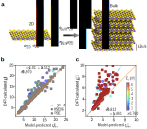
\includegraphics[width=0.9\linewidth]{img/fig4.pdf}
\caption{\label{fig-4} \textbf{Transition of dielectric properties
    from 2D to 3D systems}. \textbf{a}. Scheme for the 2D-3D
  transition. $\alpha$ in the 2D material is essentially equivalent to
  $\varepsilon$ in its bulk counterpart. \textbf{b}
  $\varepsilon_{\mathrm{bulk}}^{\parallel}$ calculated from DFT
  (y-axis) compared with the predicted value from 2D
  $\alpha_{\mathrm{2D}}^{\parallel}$ (x-axis), showing good correlation. \textbf{c}
  $\varepsilon_{\mathrm{bulk}}^{\perp}$ calculated from DFT (y-axis)
  compared with the predicted value from 2D $\alpha_{\mathrm{2D}}^{\parallel}$
  (x-axis). The predicted value is in good aggreement with the DFT
  calculation when $E_{\mathrm{g}}>4$ eV, due to minimal interlayer
  coupling. The comparisons in \textbf{b} and \textbf{c} are made
  based on both HSE06 (circles) and PBE (squares) functionals.}
\end{figure}

\begin{figure}[H]
  \centering
  \includegraphics[width=1.01\linewidth]{img/fig5.pdf}
  \caption{\textbf{Phase diagram of dielectric anisotropy $\eta$ as
      function of bandgap $E_{\mathrm{g}}$}. The
    $\eta$-$E_{\mathrm{g}}$ values of 2D materials (blue triangle) and
    their bulk counterparts (orange square) can be distinguished by
    the line $\eta=0.048(E_{\mathrm{g}}/\mathrm{eV})+0.087$. $\eta-E_{\mathrm{g}}$ values of
    semiconducting materials in other dimensions are also superimposed
    for comparison. Isotropic dielectric property is observed for bulk
    covalent materials (3D, red triangle) and fullerenes (0D, green
    star), while reduced dimensional materials, including planar
    organic semiconductor(OSc, 1D-2D, brown triangle), carbon nanotube
    (CNT, magenta circle) and linear OSc (0D-1D, violet pentagon) are
    scattered along the boundary line. The dimensionality and
    structure of typical materials are shown along the axis on the
    right. Compared with other materials, 2D materials and their bulk
    counterparts provide more flexibility of controlling the
    dielectric anisotropy.}
  \label{fig:aniso}
\end{figure}

\end{document}